\begin{figure}[h]
	
	\begin{subfigure}[b]{0.298 \textwidth}
	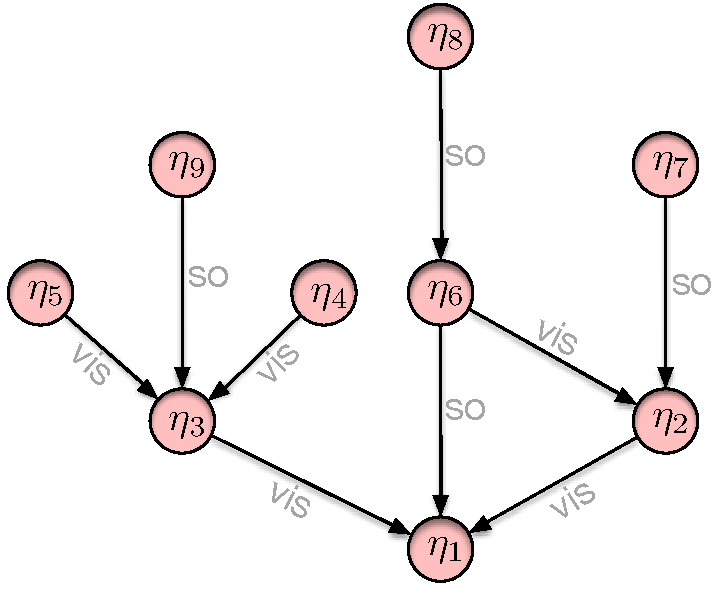
\includegraphics[scale=0.31]{Figures/execution.pdf}
	\subcaption{An execution state \E}
	\label{subfig:execution_graph}
	\end{subfigure}
	%
	\quad \vrule \quad
	%
	\begin{subfigure}[b]{0.3 \textwidth}
	\begin{smathpar}
	\scriptsize    
	\begin{array}{lcl}
	\E.\EffSoup & = & 
	\{\eta_1,\eta_2,\eta_3,\eta_4,\eta_5,\\ & & \;\eta_6,\eta_7,\eta_8,\eta_9\}\\
	\E.\visZ & = & 
	\{(\eta_5,\eta_3),(\eta_4,\eta_3),
	\\ & &\;(\eta_3,\eta_1),(\eta_2,\eta_1),	
	\\ & &\; (\eta_6,\eta_2)\} \\ 
	\E.\soZ & = & \{(\eta_9,\eta_3),(\eta_8,\eta_6),
	\\ & &\; (\eta_6,\eta_1), (\eta_8,\eta_1),
	\\ & &\; (\eta_7,\eta_2) \} 
	\end{array}
	\end{smathpar}
	\subcaption{Effect soup and primitive relations}
	\label{subfig:execution_example}
	\end{subfigure}
	%
	\quad \vrule \quad
	%
	\begin{subfigure}[b]{0.26 \textwidth}
	\begin{smathpar}
	\scriptsize
	\begin{array}{lll}
	\visZ^{-1}  (\eta_1) & = & \{\eta_2,\eta_3\} \\ 
	\soZ^{-1}  (\eta_1) & = & \{\eta_6, \eta_8\} \\
	(\soZ\cup\visZ)^{-1} (\eta_1) & = &
	\{\eta_2,\eta_3, 
	\eta_6,\eta_8\} \\ 
	(\visZ^*)^{-1} (\eta_1) & = &
	\{\eta_2,\eta_3,\eta_4,\eta_5,\eta_6\} \\ 
	(\soZ;\visZ)^{-1}(\eta_1) & = & \{\eta_7,\eta_9\}
	
	\end{array}
	\end{smathpar} \\
	\subcaption{Relation inverse examples}
	\label{subfig:inverse_example}
	\end{subfigure}
	\caption{A simple execution state }
\label{fig:execution_state}
\end{figure}
